\documentclass[titlepage]{article}
\usepackage[a4paper, total={6in, 8in}]{geometry}
\usepackage[utf8]{inputenc}
\usepackage{graphicx}
\usepackage{hyperref}
\usepackage[section]{placeins} % stop floating figures from going in the wrong sections
\usepackage[toc]{glossaries}


\newglossaryentry{Domain}
{
  name=Domain,
  description={The scope of things and their properties that are of interest for an application.
In YODA, a domain is formalized through an ontology.}
}


\newglossaryentry{Ontology}
{
  name=Ontology,
  description={A formal, written description of a domain. 
Typically this includes information such as a class hierarchy and the set and type restrictions of predicates.
In YODA, a system's domain is specified with an ontology built by extending some core Java classes.}
}


\newglossaryentry{ASR - Automated Speech Recognition}
{
  name=ASR - Automated Speech Recognition,
  description={A computer program that takes raw audio signals as input and delivers a sequence of words as output.
YODA does not provide an ASR component.}
}

\newglossaryentry{SLU - Spoken Language Understanding}
{
  name=SLU - Spoken Language Understanding,
  description={A computer program that takes a sequence of words as input and delivers some semantic representation as output.
This can be a set of slot-value pairs (known as shallow SLU), or a structured logical representation (as in the SLU component in YODA).}
}

\newglossaryentry{TTS - Text To Speech}
{
  name=TTS - Text To Speech,
  description={A computer program that takes a sequence of words as input and delivers audio of those words being spoken as output.
This is often the last module in a spoken dialog system pipeline.
YODA does not provide a TTS engine.}
}

\newglossaryentry{FOL - First Order Logic}
{
  name=FOL - First Order Logic,
  description={A formalism for describing a state of belief and concluding other beliefs through proof.}
}

\newglossaryentry{KB - Knowledge Base}
{
  name=KB - Knowledge Base,
  description={A portion of computer memory which contains a logical model of what a program knows.}
}





\makeglossaries

\hypersetup{
    colorlinks=true,       % false: boxed links; true: colored links
    linkcolor=red,          % color of internal links (change box color with linkbordercolor)
    citecolor=green,        % color of links to bibliography
    filecolor=magenta,      % color of file links
    urlcolor=blue           % color of external links
}


\title{YODA Tutorial}
\author{David Cohen }
\date{\today}



% \makeglossaries

% \newglossaryentry{latex}
% {
%     name=latex,
%     description={Is a mark up language specially suited 
%     for scientific documents}
% }
 
% \newglossaryentry{maths}
% {
%     name=mathematics,
%     description={Mathematics is what mathematicians do}
% }

\begin{document}


\maketitle

\tableofcontents

\begin{abstract}
This tutorial introduces the YODA architecture at a high level, then walks through some of the basic features of the YODA dialog system architecture through an example Smart Home application.
\end{abstract}



\section{What is YODA and Who Should Use it?}

YODA is a spoken dialog system architecture - a piece of software to enable the creation of spoken dialog systems for various purposes, in various domains.
Below are two check-lists that might help determine if YODA is right for you.\\


\noindent
YODA may be good for you if some of these points describe your situation:
\begin{itemize}
  \item You want to build an application where users can talk to a computer in a way where it remembers the context of what they've been talking about from turn to turn, allowing them to speak naturally and not specify every detail of what they mean.
  \item You do not have a large annotated data set of dialogs in your chosen domain / you do not have the money to buy one / you do not have the expertise to know what to collect / you do not have the time to wait while this all happens.
  \item Your domain has a dynamic set of objects about which your system needs to fluently converse.
  \item You want your system to be able to answer questions and follow commands related to the things it knows about in your domain.
  \item You want to have a working dialog system \textbf{fast}.
  \item You do not want a dialog system that evades questions it doesn't understand, acts like it understands things it doesn't, and tries to get the user to do all the work - like the classical Eliza therapist or a chat bot.
\end{itemize}

\noindent
YODA, in its current state, may not be good for you if any of these things describe your situation:
\begin{itemize}
  \item You don't trust any software tool that admits to requiring developers to ``engineer knowledge'' (YODA admits to this).
  \item You can't work with the GPL3 license.
  \item You have an unlimited fountain of money, data, and expertise which you plan to bring to bear on your specific dialog project.
  \item Your engineers (and their bosses) must exercise complete control over what the system says to create a user experience aligned with business objectives.
  \item You have some weird problem with the Java programming language.
\end{itemize}




\section{YODA Overview}

\subsection{Logical Knowledge-base-centric Agents}

A YODA dialog system is an agent in the tradition of other logical-knowledge-base-centric agents, as shown in figure \ref{logical-kb-agent}.
The agent acts upon the world, and updates its world model based on input from sensors.

\begin{figure}[h!]
\centering
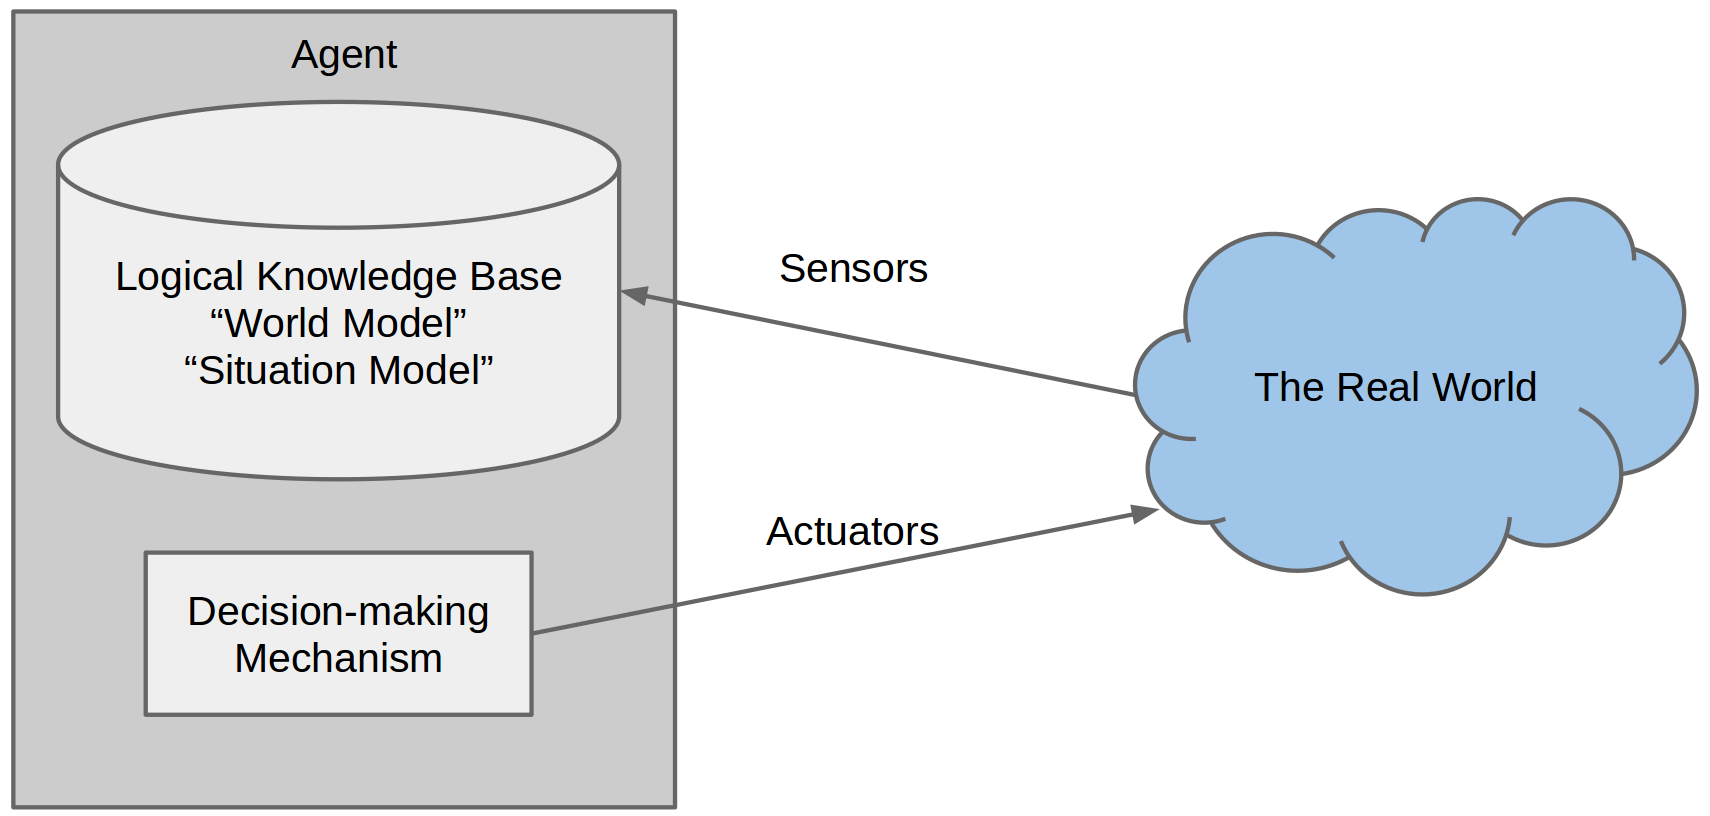
\includegraphics[width=.75\textwidth]{logical_kb_agent}
\caption{Logical KB-based system.}
\label{logical-kb-agent}
\end{figure}

YODA presupposes that dialog state tracking information and inferences are different enough from other types of inference and belief maintenance that they should be performed by separate modules.
Particularly, speech recognition and understanding are highly specialized sensing operations.
Figure \ref{separated-logical-kb-agent} shows a more accurate model of how YODA models its own position in the world.
As is shown in the figure, YODA uses a separate representation for dialog state then it does for its world / situation (terms used interchangeably) model.
The world model is a Sesame RDF datastore with forward-chaining inferencing.
The dialog state model is set of Java objects describing a distribution of the possible `histories of things said' by the user and system in the dialog up to the current moment.

\begin{figure}[h!]
\centering
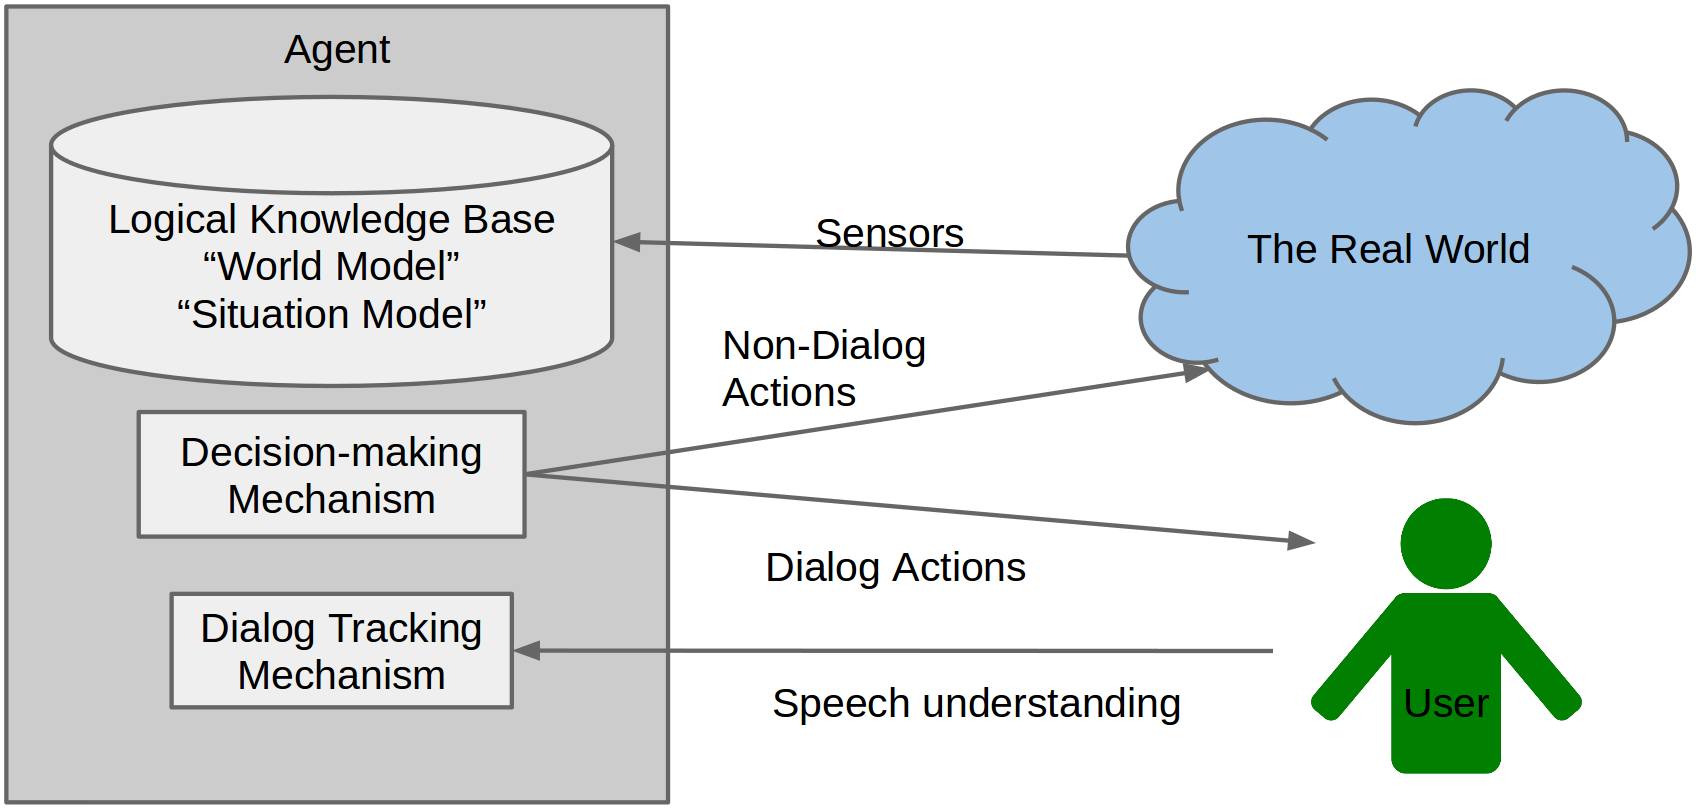
\includegraphics[width=.75\textwidth]{separate_dialog}
\caption{Separating the dialog component from a logical KB-based system.}
\label{separated-logical-kb-agent}
\end{figure}

\subsection{Ontology as Architectural Glue}


YODA is an ontology-driven architecture, which means it is able to discuss and interact to communicate information about world entities so long as the developer describes the relevant entities in a suitable knowledge structure a.k.a. ontology.

A YODA dialog system's ontology acts as `architectural glue' by specifying how all the other components can behave and interact with each other.
A YODA system's ontology does these things (and more):
\begin{itemize}
\item Language semantics (SLU valid outputs / NLG valid inputs) are restricted by the ontology.
\item Dialog pragmatics modelling and inference (done by the Dialog State Tracking module) are restricted by the ontology.
\item The system's world model (database) is limited by the ontology, and the ontology defines how that database should be interpreted.
\item Actions considered by the dialog manager have parameters which are limited by the ontology.
\item Interfaces to non-dialog tasks and sensors are built on the system ontology.
\end{itemize}

YODA provides a skeleton ontology, and a system engineer extends the ontology with classes that are specific to their domain.
Domain ontology classes are defined as Java classes, as is detailed later in this tutorial.

\subsection{Dialog with YODA}

Many dialog systems operate by generating plausible statements and responses to keep the dialog going, in the spirit of the Eliza computer therapist or a chat-bot that attempts to pass the Turing Test.
The purpose of these dialog systems tends to be to keep the user engaged, possibly while guiding them through a tree-like dialog structure to perform some task.
Often, these systems have built-in strategies for ignoring the users when they ask things the system does not understand, and subtly directing the user back to the prescribed dialog tree. 
Supporting this type of dialog system is \textbf{not} the purpose of a YODA.

YODA attempts to enable dialog systems which actually understand their users within the scope of a domain, and respond in common helpful ways: by answering questions and obeying commands.
Users will hopefully use dialog systems built with YODA because of their utility, naturalness of use, and because they are transparent and not misleading about their intelligence and capabilities.

\section{Building a YODA System - Overview}

Building a basic dialog system on top of the YODA architecture is a fairly simple process, consisting of the following steps:

\begin{enumerate}
  \item Build and register databases
  \item Implement and register sensors
  \item Implement and register non-dialog tasks
  \item Build and register domain ontology
  \item Provide a lexicon
  \item Extend a YODA executable to include the new domain
\end{enumerate}

This tutorial will explain the smart house demo system built on top of YODA.
The purpose of this system is to allow a user to use, for example, a smart-phone app to stay informed about the state of their house and command various appliances remotely.
The full source code for this system along with the source for several other demonstration systems, is available as part of YODA.

\section{Build and Register Databases}
YODA reads databases in \href{http://www.w3.org/TeamSubmission/turtle/}{rdf turtle format}.
Databases should capture the static / initial knowledge of a system.
The contents of a registered database are loaded during system start-up, and the turtle file is never modified, but the facts listed in the database may change in the running system's working memory as a result of sensing.

Figure \ref{fig:smart_house_database} shows the turtle file used to describe the initial smart house situation.
There are a few appliances, rooms and people that make up the initial situation.

\begin{figure}[h!]
\centering
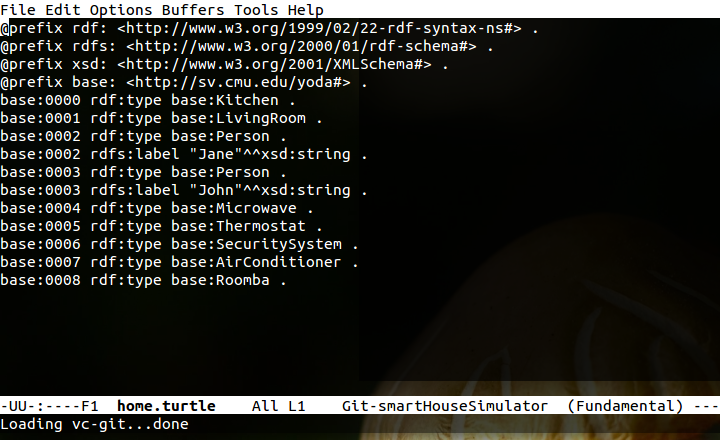
\includegraphics[width=.75\textwidth]{SmartHouseDatabase}
\caption{The rdf database file home.turtle describes the initial situation in the smart home demo system.}
\label{fig:smart_house_database}
\end{figure}

Some important things to remember while writing a database:
\begin{itemize}
\item Remember to include common prefixes in the header of your turtle file, as well as the yoda prefix (these are lines 1-4 in the example).
\item Every `entity' or `individual' should have a unique identifier called a URI (Universal Resource Identifier). Most likely, these individuals should have a prefix of `base:'. In the smart house example, there are 9 unique individuals, numbered 0000 to 0008. Don't confuse the URI with the `name' or other information about an individual that may not be unique.
\item Every entity should have a type, defined using the rdf:type predicate. If the system is supposed to be able to talk about this entity, it should be a type which inherits from the YODA skeleton ontology class Noun, and is registered in your ontology (see later section for how to do this). Examples in this turtle database file include base:Kitchen, base:LivingRoom, base:Person, base:Microwave, base:Thermostat, base:SecuritySystem, base:AirConditioner, and base:Roomba.
\item Remember to register the database in the database registry file. This is demonstrated in the third line of code from Figure \ref{fig:sensor-example}.
\end{itemize}



\section{Build and Register Sensors}

Sensors are an agent's continual inputs, which allow it to maintain an up-to-date model of the world's state.
YODA provides a sensor interface which the developer can implement in their own system.
Sensors are called at approximately 10Hz, soon the interface will be extended to allow for lower-period sensing.


\begin{figure}[h!]
\centering
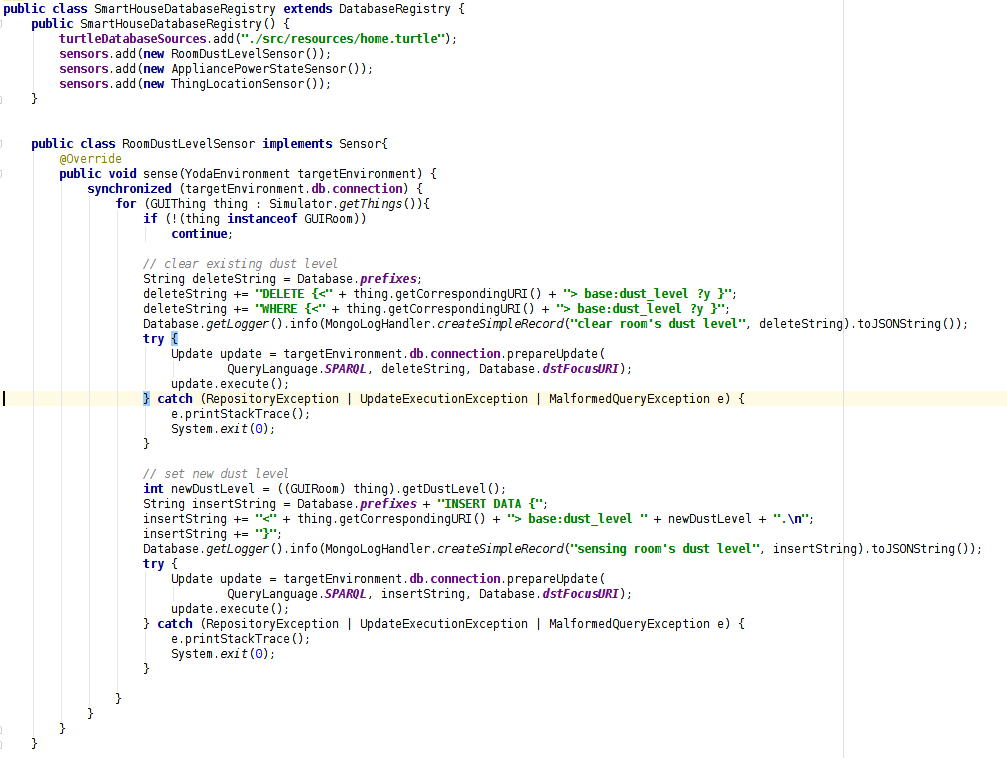
\includegraphics[width=\textwidth]{smart_house_sensor_example}
\caption{An example from the smart house database registry, including an example sensor implementation which senses room dust level.}
\label{fig:sensor-example}
\end{figure}


Figure \ref{fig:sensor-example} is an excerpt from SmartHouseDatabaseRegistry.java, the database and sensor registry for the smart house demo system.
The current sensor interface requires the developer to directly update the system's database via SPARQL DELETE and INSERT operations.
As the example illustrates, this typically involves deleting facts that are currently in the database, and replacing them with updated facts.
The smart house demo system includes a home simulator, and the new facts are pulled from there; however, in a real system, these facts will be determined from various real-world sensors.
This example includes the sensor for detecting room dust levels, but as is apparent, there are two other sensors registered: one to detect appliances' power states, and another to detect the location of things in the house.

Some important things to remember while writing a sensor:
\begin{itemize}
\item Synchronize the database connection so that the system does not attempt to query the database contents while they're being changed.
\item Delete old facts, then add new facts. Adding new facts that contradict will not delete old facts, it will create a contradictory world model.
\item Register sensors in the database registry (add them to the "sensors" member variable).
\end{itemize}



\section{Implement and Register Non-Dialog Tasks}

TODO: UPDATE THIS SECTION (describe the simulator here)

If a YODA dialog system is to do more than answer questions, the developer needs to implement some non-dialog tasks and register them with the system.
Figure \ref{fig:turn_on_task} shows the important parts of the implementation we use for this demo.
The TurnOnTask non-dialog task 'turns on' an appliance by directly modifying the database.
Of course, in the real world, these tasks should have real-world effects, and sensors should update the database, but this works for demonstration purposes.


\begin{figure}[htbp!]
\centering
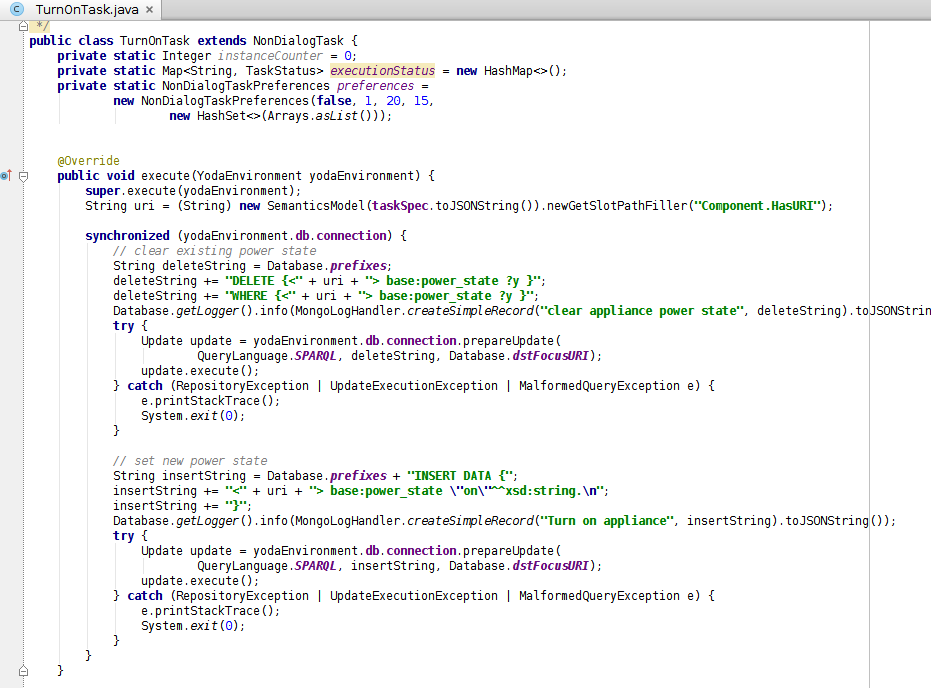
\includegraphics[width=\textwidth]{TurnOnTask}
\caption{A sample non-dialog task - TurnOnTask turns on an appliance by directly modifying the database.}
\label{fig:turn_on_task}
\end{figure}

Figure \ref{fig:non_dialog_task_registry} shows the class that registers TurnOnTask and uses the standard Command template to map the TurnOnAppliance verb to the task specification.


\begin{figure}[htbp!]
\centering
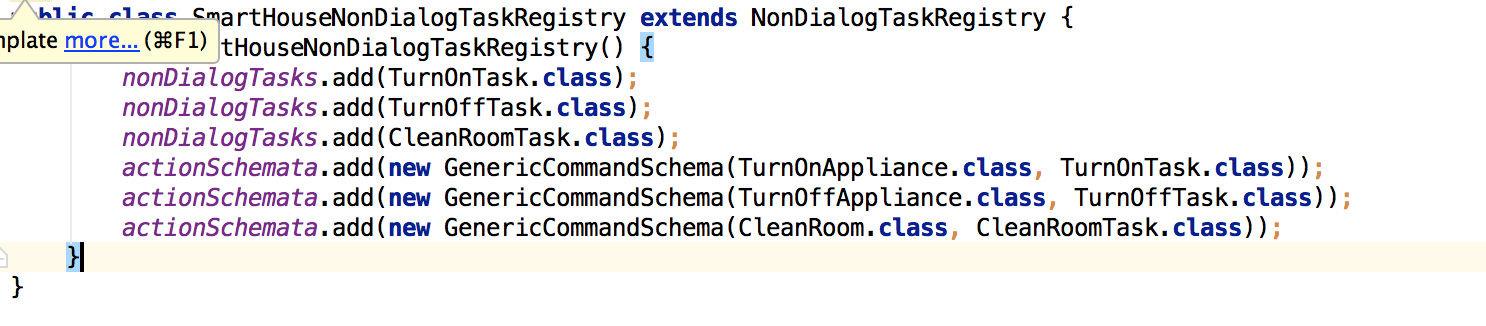
\includegraphics[width=\textwidth]{NonDialogTaskRegistry}
\caption{The smart home non-dialog task registry.}
\label{fig:non_dialog_task_registry}
\end{figure}

\section{Build and Register a Domain Ontology}

YODA provides a skeleton ontology, and a system developer should extend it for their own task.
The major base classes are Noun, Verb, Role, TransientQuality, Adjective and Preposition, and some examples are given in the following sub-sections of extensions of these base classes for the smart house domain.
Whenever you add a new class to the ontology, you need to tell the ontology registry that that class exists (it doesn't automatically add all the classes it can find, to allow for quicker experimentation with different ontology designs).
The ontology registry for the smart house domain is shown in Figure \ref{fig:smart_house_ontology_registry}.

\begin{figure}[h!]
\centering
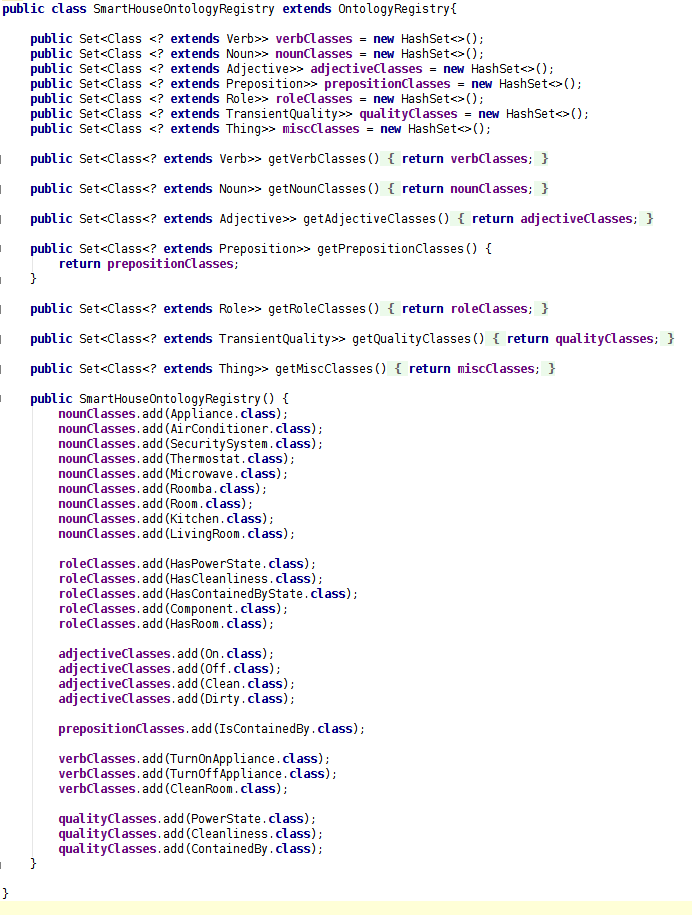
\includegraphics[width=.75\textwidth]{OntologyRegistry}
\caption{SmartDomainOntologyRegistry.java, registering the domain ontology with YODA.}
\label{fig:smart_house_ontology_registry}
\end{figure}

An ontology registry for any other domain should include identical boilerplate code as this example, and the domain-specific classes should be added to the registry as part of the constructor.
There is no need to re-register classes from the skeleton ontology, the skeleton ontology has its own registry, which will be included later.

Some advice when working on your ontology:
\begin{itemize}
\item Test as you go. 
Build related ontology items, lexicon entries, database entries and sensors together and test them together. 
Otherwise, there will inevitably be errors which are difficult to locate.
\item Remember to \textbf{register your ontology classes} as you create them.
\end{itemize}


\subsection{Noun}
Nouns are the concepts which we usually describe as nouns in language - particularly the physical and abstract objects which make up a domain.
There is not much work to do to define a noun, simply create a Java class that inherits from the appropriate parent within the Noun sub-tree.
Two examples are shown in Figure \ref{fig:nouns}.
Appliance is a high-level class, which inherits from the YODA skeleton ontology's PhysicalNoun class.
AirConditioner is a more specific appliance sub-class, so it inherits from Appliance.

\begin{figure}[!]
\centering
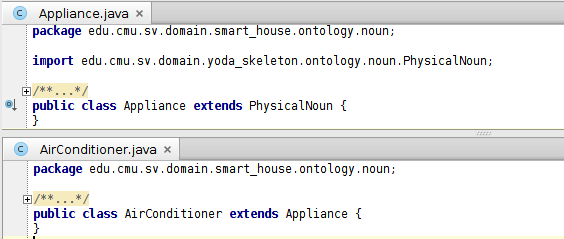
\includegraphics[width=.75\textwidth]{Nouns}
\caption{Two Java classes to define two ontology Noun classes.}
\label{fig:nouns}
\end{figure}



\subsection{Transient Qualities, Adjectives and Prepositions}

A dialog system needs to be able to determine to what degree an entity matches a description (reference resolution), and generate unambiguous descriptions to refer to objects (reference generation).
For example, if the user asks the smart house dialog system ``Is the kitchen dirty?'', the dialog system needs to figure out what ``the kitchen'' is referring to, and whether that thing is dirty.
Similarly, if there are multiple entities in the discourse (as there usually are), and the system needs to describe one of them, it might select some quality which disambiguates its true referent from the other possibilities.
To get the most out of YODA's support for this, a developer is required to implement transient qualities and the corresponding adjectives and prepositions that make up their domain.\\

\subsubsection{Overview}

Adjectives and prepositions are `grouped' by the quality which maps to them. 
For example, the adjectives `cheap' and `expensive' are grouped with the quality `price range', and the prepositions `close to' and `far from' are grouped with the quality `distance'.
The basic relationship between qualities and adjectives / prepositions, along with the basic procedure for inferring the truth value of any one adjective / preposition are shown in Figure \ref{fig:quality_computation}.
The system's database encodes everything it needs to determine whether an adjective / preposition holds.
The system runs a SPARQL query on the database to determine the quality's degree, then applies a piecewise linear map to determine the truth degree of the adjective / preposition.


\begin{figure}[h!]
\centering
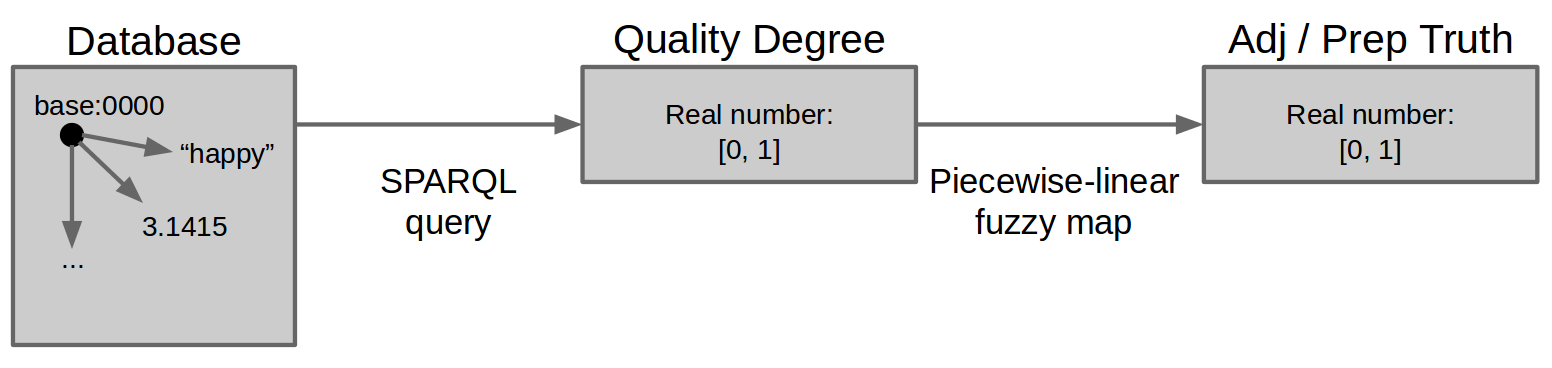
\includegraphics[width=\textwidth]{QualityComputation}
\caption{Diagram of the procedure to compute the truth value of some adjective w.r.t an entity or some preposition w.r.t. two entities.}
\label{fig:quality_computation}
\end{figure}


Specifying the query to run is part of defining a custom TransientQuality in the ontology, while parameterizing the piecewise linear mapping is part of defining a custom Adjective / Preposition in the ontology.


% The standard first-order logic representation of some entity $x$ being described by an adjective $A$ is: $A(x)$, and if some relationship $B$ holds between a pair of entities, $x$ and $y$, the FOL representation would be $B(x,y)$.
% These facts, once added to an agent's logical KB, could be used to infer other facts, or make decisions.
% There are several major flaws with this representation.
% First, many adjectives and prepositions are subjective.
% For example, we might say a restaurant is `cheap', but that statement is probably an assessment based on the prices of some items on their menu relative to comparable menu items at other restaurants in the speaker's experience.
% Second, cheapness has degrees.
% A restaurant can be free, cheap, sort of cheap, or not cheap.
% Third, `cheap' is closely related to another adjective `expensive', in that they both seem to be determined from the same underlying information.
% This fact should be easy to encode.

\noindent To enable YODA to make use of a group of related adjectives or prepositions for reference resolution and generation, the developer needs to do the following:
\begin{itemize}
\item Extend TransientQuality to create a new quality, implement its getQualityCalculatorSPARQLQuery() method.
\item Define an adjective or preposition `group' by extending Adjective or Preposition (depending on whether your quality is unary or binary) with a new abstract class which will encapsulate all the adjectives and prepositions in this group, and implement its getQuality() method.
\item Extend Adjective or Preposition and override getCenter() and getSlope() for each adjective / preposition in the group.
\item Extend HasQualityRole with a new role and give it a domain and range appropriate for the new quality.
\item Register all of these ontology classes!
\end{itemize}


\subsubsection{Extending TransientQuality}

Every custom TransientQuality will need to override the getQualityCalculatorSPARQLQuery().
This method returns a function which generates part of a SPARQL query given a list of arguments.
If the quality is unary (for adjectives), there will be two arguments: the first argument is the entity who the quality is being determined for, and the last argument is the variable which should have the result bound to it.
If the quality is binary (for prepositions), there will be three arguments: the first two are the entities which the quality is being determined for, and the last argument is the variable which should have the result bound to it.

The implementation of getQualityCalculatorSPARQLQuery() depends intimately on how the quality is sensed / encoded in the database.
This subsection presents two examples which a large fraction of anticipated use cases will resemble.
There are several other TransientQuality implementations included in the smart house and Yelp Phoenix demo systems, which you should use as additional references.


A simple example from the smart house domain is the Cleanliness unary quality, which supports the Clean and Dirty adjectives.
Figure \ref{fig:cleanliness_quality} shows the ontology definition of the Cleanliness quality.
The smart home system has some way of sensing the dust level of rooms within the house, and it is encoded as an integer from 0 to 5 using the base:dust\_level predicate.
The SPARQL query in this example maps that to the range between 0 and 1, where 1 is higher cleanliness by taking $1.0 - 0.2 * d$ where $d$ is the dust level.
This way, if the dust level is $0$, then Cleanliness is $1$.

\begin{figure}[h!]
\centering
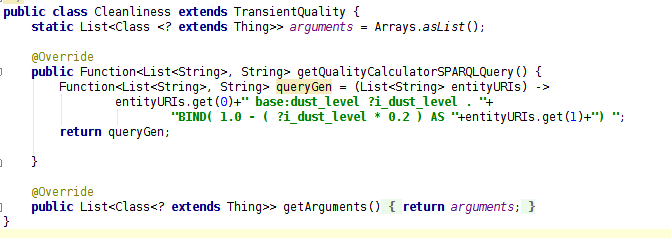
\includegraphics[width=\textwidth]{CleanlinessQuality}
\caption{Ontology definition of the Cleanliness TransientQuality.
This quality is later mapped to the Clean and Dirty adjectives.
The definition includes a SPARQL query which determines a float value between 0 and 1, which is the ``degree of cleanliness'' for an input individual.}
\label{fig:cleanliness_quality}
\end{figure}


A more complicated example is the ContainedBy quality, which supports the preposition IsContainedBy (relating things to the room that contains them).
The ontology definition of ContainedBy is shown in Figure \ref{fig:contained_by}.
In this case, the quality can basically be determined as an objective fact from the database; the base:in\_room predicate relates the thing to the room which contains it.
Unfortunately, the SPARQL code to map this to $0$ and $1$ is a bit cryptic, which is why I've included the example.
Since this is a binary quality, which relates two entities, the input list of entity URIs is longer than for a unary quality.\\

\begin{figure}[h!]
\centering
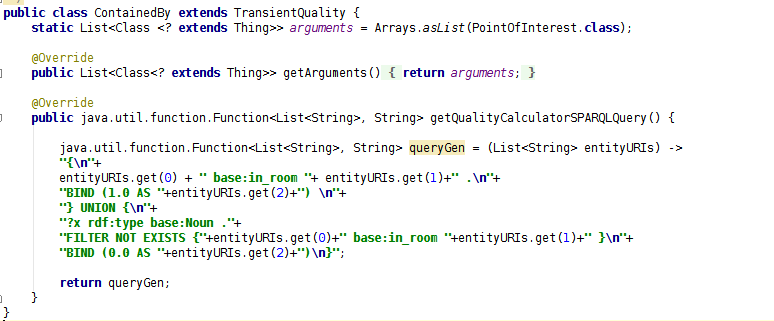
\includegraphics[width=\textwidth]{ContainedByQuality}
\caption{Ontology definition of the ContainedBy TransientQuality.
This quality is later mapped to the IsContainedBy preposition, which relates an appliance or person to the room in the house that it is in.}
\label{fig:contained_by}
\end{figure}



\noindent Some notes for extending TransientQuality:
\begin{itemize}
\item Look through all the available example implementations to see if your use case closely resembles them.
\item Use the sparql\_playground git repository to edit a turtle file and try out your own queries in a simpler environment than a full-fledged YODA dialog system.
\item Implement the static ``arguments'' boilerplate, which should be an empty list for unary qualities, and should be the type of Noun being related to for binary qualities. Also override the getArguments() method.
\end{itemize}


\subsubsection{Defining Adjective / Preposition Groups}

Frequently several related adjectives / prepositions are mapped from the same quality.
In this case, it reduces required boilerplate to create a single abstract adjective / preposition class, and to make all the concrete classes inherit from it.
Figure \ref{fig:group_abstract_adjective} shows the group class for the adjectives derived from the Cleanliness quality.
Make sure to override the getQuality() method to return the appropriate quality class.

\begin{figure}[h!]
\centering
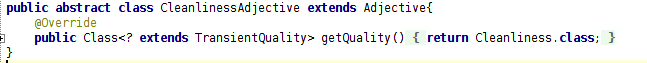
\includegraphics[width=\textwidth]{GroupAbstractAdjective}
\caption{Ontology definition of the CleanlinessAdjective group.
This is an abstract class, but still must be registered with the ontology.}
\label{fig:group_abstract_adjective}
\end{figure}


\subsubsection{Adding Custom Adjectives / Prepositions}

Once the quality and group have been defined, all that needs to be done to define a custom adjective / preposition is:
\begin{itemize}
\item Extend the abstract group class with the custom adjective / preposition.
\item Overwrite getCenter() and getSlope() to specify the linear fuzzy map for the given adjective / preposition relative to the group's quality.
\end{itemize}

The piecewise linear fuzzy map is a function which maps a quality degree to an adjective / preposition truth.
It is a pyramid function with value 1 at the center, and sloping downward in both directions until bottoming out at zero.
The resulting truths are also in the range [0,1].

\begin{figure}[h!]
\centering
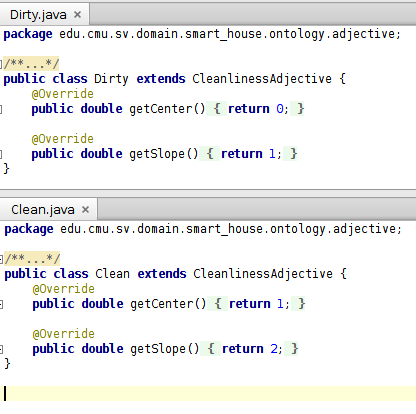
\includegraphics[width=.6\textwidth]{CleanAndDirty}
\caption{Ontology definitions of Clean and Dirty.
Notably, these inherit from the group's abstract adjective class, and include parameters for the piecewise linear map from Cleanliness.}
\label{fig:clean_and_dirty_definition}
\end{figure}


\begin{figure}[h!]
\centering
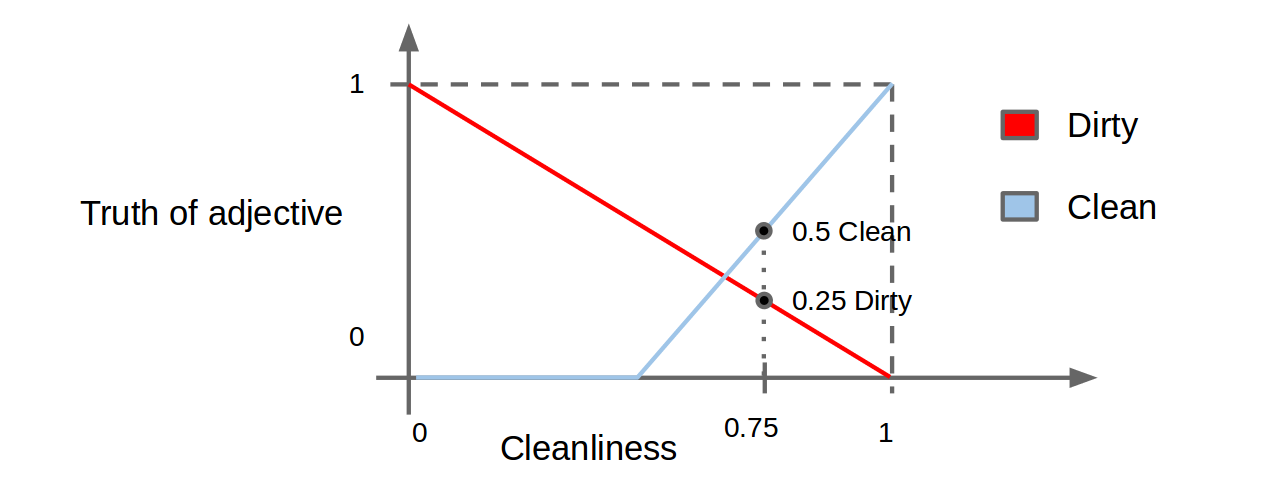
\includegraphics[width=\textwidth]{CleanDirtyFuzzyMap}
\caption{Piecewise-linear fuzzy mapping from the Cleanliness transient quality to the Clean and Dirty adjectives. 
When the degree of Cleanliness is .75, then Clean is .5 true, and Dirty is .25 true.
Drawn in red and blue are the piecewise-linear mapping functions, which are parametrized by a center point and a slope downward from that center point.}
\label{fig:clean_dirty_fuzzy_map}
\end{figure}

Figure \ref{fig:clean_and_dirty_definition} shows the definitions of the Dirty and Clean adjectives.
Notably, these inherit from the group's abstract adjective class, and include parameters for the piecewise linear map from Cleanliness.
The fuzzy maps for these two adjectives are illustrated in Figure \ref{fig:clean_dirty_fuzzy_map}.
As the figure shows, Clean has a higher slope than dirty, and it will have a truth value of $0$ for any Cleanliness value $<= 0.5$.
The choice of center and slope are somewhat arbitrary, and they depend on what scale the quality itself has.
Ideally, choosing parameters should be an empirical task based on measuring the quality when adjectives are used by people.


\subsubsection{Adding Roles and Registering}

Roles need to be added for completeness.
For every adjective or preposition group, you need to implement a HasQualityRole that acts as a semantic connector between nouns and the group.
An example for the Cleanliness adjective group is shown in Figure \ref{fig:has_cleanliness_role}.

\begin{figure}[h!]
\centering
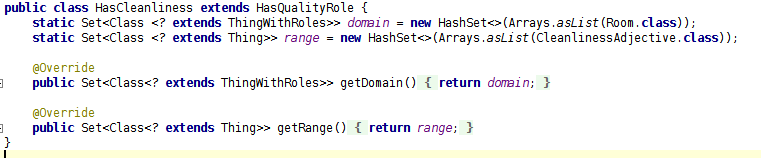
\includegraphics[width=\textwidth]{HasCleanlinessRole}
\caption{The HasCleanlinessRole is the semantic connector between nouns and cleanliness adjectives.}
\label{fig:has_cleanliness_role}
\end{figure}



\subsection{Role}
Roles are relations between two entities

\subsection{Verb}
This domain defines one new verb TurnOnAppliance, which is used to issue commands.
Figure \ref{fig:turn_on_appliance} shows the class definition, which includes a list of required grounded roles.
TurnOnAppliance is not considered semantically complete unless the Component role has been provided.
This information is used to guide slot-filling dialog and to help the system decide when to ground certain noun phrases.
In the non-dialog task registry, we later specify that the standard mapping is used to turn command dialog acts containing the TurnOnAppliance verb into the TurnOnTask non-dialog task.
This is discussed in a later section.

\begin{figure}[h!]
\centering
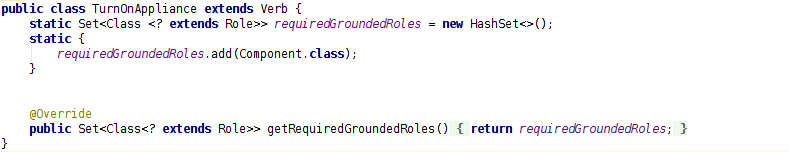
\includegraphics[width=\textwidth]{TurnOnAppliance}
\caption{Definition for the TurnOnAppliance verb.}
\label{fig:turn_on_appliance}
\end{figure}

\section{Provide a lexicon}

TODO: UPDATE THIS SECTION


YODA's NLG and SLU components rely on a developer-provided lexicon, which provides words and phrases to represent the different ontology concepts in different parts of speech.
Figure \ref{fig:lexicon} shows the lexicon used in the smart home tutorial.
Both the NLG and SLU components make use of the information in the lexicon.
Often, we want our system to use formal words for generation, but to understand humans in whatever words they choose.
Accordingly, we can add a word to the lexicon for understanding but not for generation by setting the third parameter of the Lexicon.add() function to `true'.
In this case, the term "power up" will be understood by the system, but not generated.

\begin{figure}[h!]
\centering
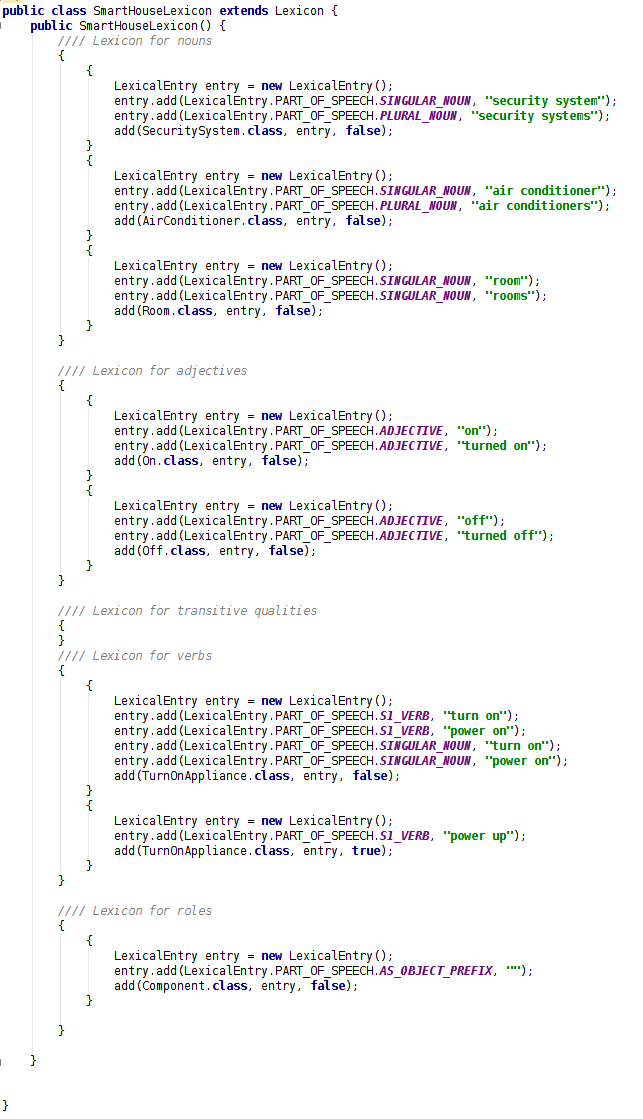
\includegraphics[height=.95\textheight]{Lexicon}
\caption{The lexicon used to power the SLU and NLG in the smart home demo system.}
\label{fig:lexicon}
\end{figure}


\section{Extend a YODA Executable}

TODO: UPDATE THIS SECTION: include a more exciting example from the current system

The final step of creating a YODA dialog system is to extend one of the provided executable dialog systems to include the new domain.
Figure \ref{fig:smart_house_command_line_system} shows the executable which includes the smart house domain.
All that is required in the executable is to extend a YODA base executable and add the yoda skeleton domain and the smart house domain in a static context.

\begin{figure}[h!]
\centering
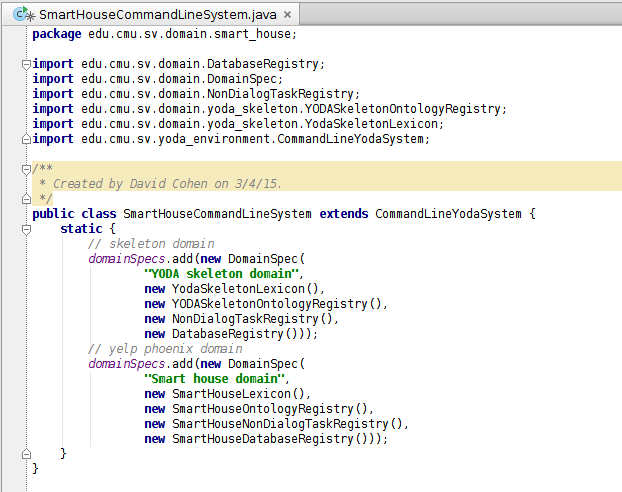
\includegraphics[width=\textwidth]{SmartHouseCommandLineExecutable}
\caption{SmartHouseCommandLineSystem.java is a fully-functioning command line dialog system in the smart house domain.}
\label{fig:smart_house_command_line_system}
\end{figure}

This creates a command-line dialog system, which takes words as input, and outputs words (and non-dialog tasks).
An example dialog with this system is shown in Figure \ref{fig:smart_house_demo}.

\begin{figure}[h!]
\centering
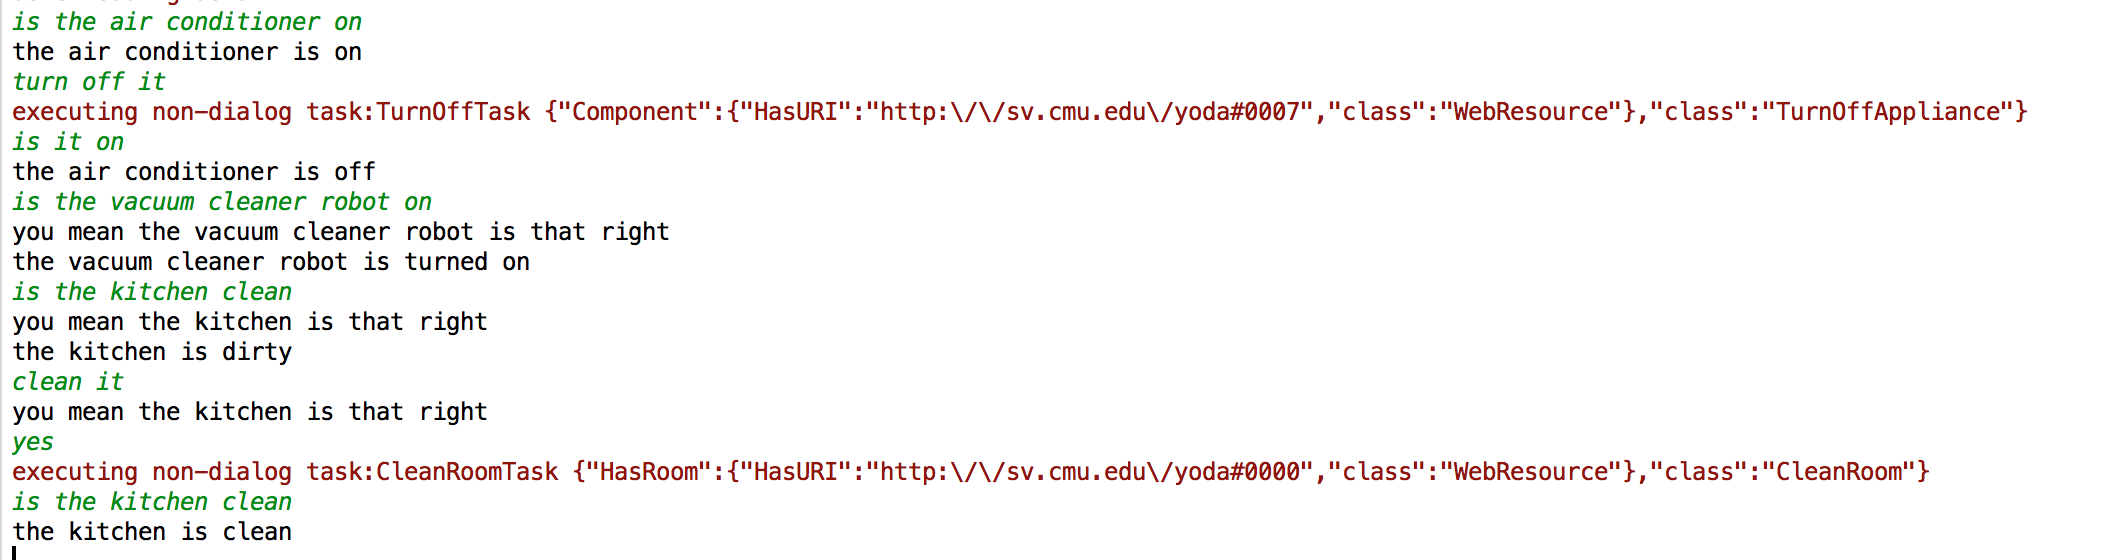
\includegraphics[width=\textwidth]{SmartHouseDemoDialog}
\caption{A sample dialog with the program SmartHouseCommandLineSystem.java.}
\label{fig:smart_house_demo}
\end{figure}


\clearpage
\glsaddall
\printglossary[type=main,nonumberlist]


\end{document}
